\chapter{Einbettung in Gaia-X kompatible Cloud}
\label{chapter:gaia-x-einbettung}
Gaia-X ermöglicht und fördert die Bildung von Föderationen.
Föderationen dienen als eigenständige Ökosysteme, in denen sich einzelne Teilnehmer zusammenschließen können,
um Services innerhalb oder auch außerhalb der Förderation anzubieten, um Teilnehmern einen Mehrwert zu bieten \cite{GXFS2021}.
Gaia-X operiert nicht, wie alleinstehende Cloud-Providerfirmen, selbst auf dem Markt, sondern erstellt
Software Komponenten zur Erstellung eines föderalisierten Systems in dem mehrere Teilnehmer
untereinander kommunizieren und interagieren können \cite{GXFS2021}.
Als einer der ersten Testimplementationen für Gaia-X gilt die Pluscloud Open,
welche auf Basis des Open Source Projekts \ac{SCS} läuft.
Zum Zweck dieser Arbeit wurde eine zeitlich begrenzte Testlizenz bereitgestellt,
welche die Möglichkeit bietet, die in dieser Arbeit erstellte Referenzimplementation
in einer Gaia-X kompatiblen Umgebung zu testen.


\section{Bereitstellung im Gaia-X Katalog}
\label{sec:gaia-x-einbettung:gaia-x-katalog}
Gaia-X definiert in den Föderationsservices einen Service Katalog, in dem Anbieter Services registrieren
und Konsumenten mittels Suchalgorithmen einen Service für ihre Bedürfnisse finden können \cite{GaiaXArchitecture2021}.
Im Katalog bereitgestellte Services müssen den Nutzer informieren, welche Eigenschaften der jeweilige Service besitzt.
Dadurch können Endnutzer auswählen, welche Services in welchem Standardort 
und zu welchen Umständen, wie die Nutzung des Bereitstellungstools, Betrieb des Service etc. sie nutzen möchten.
Dieses Prinzip wird in Gaia-X \emph{Self-Description} genannt.
Self-Descriptions werden mittels JSON-LD dargestellt, ein
leichtgewichtiges \emph{Linked Data} Format \cite{Eggers2020}.
Betreiber eines Service sind dabei selbst für die Erstellung einer \emph{Self-Description} verantworlich \cite{GaiaXArchitecture2021}.

\begin{figure}
  \centering
  \makebox[\textwidth][c]{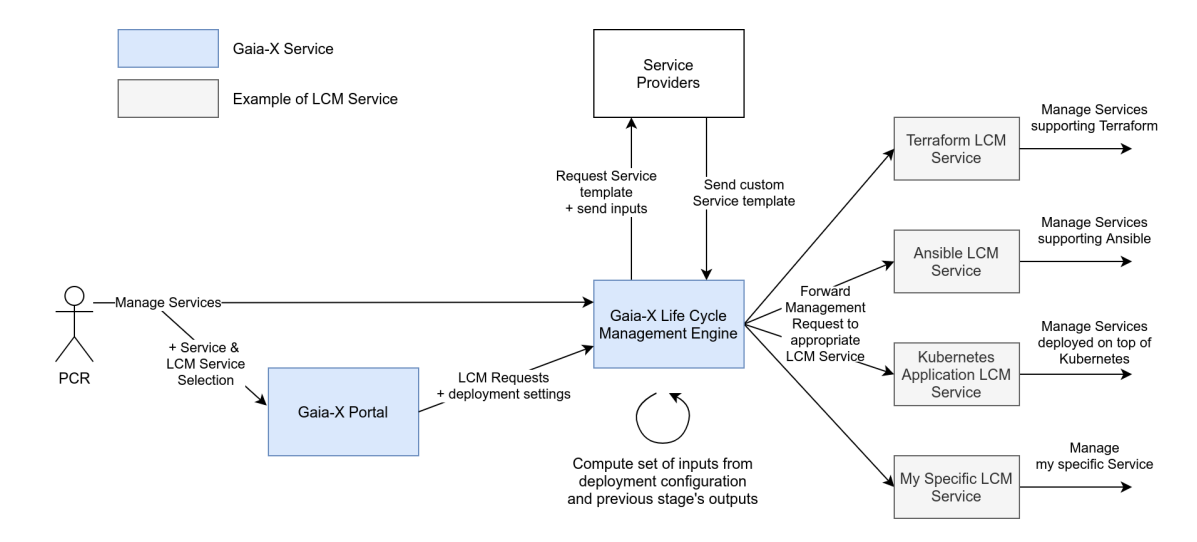
\includegraphics[width=1.35\textwidth]{gfx/chapters/4_gaia-X/orchestration_overview.png}}
  \caption{High Level Übersicht für Gaia-X Service Bereitstellung}
  \source{\cite{ORC2021}}
  \label{fig:gaia-x-orchestration-overview}
\end{figure}

In \ref{fig:gaia-x-orchestration-overview} wird die Kommunikation innerhalb Gaia-X Akteuren
zur Bereitstellung von Services in Gaia-X dargestellt.
Die \ac{LCM} Engine dient als Einstiegspunkt für Kommunikation mit dem Endnutzer. 
Jegliche Verwaltungsanfragen für Services werden an sie gestellt.
 Die Engine verteilt daraufhin diese Anfragen
an den jeweiligen Bereitstellungsservice anhand der Auswahl des Nutzers \cite{ORC2021}.
Im Architekturbild übernimmt die in dieser Arbeit erstellte Referenzimplementation
den Teil des \emph{Kubernetes Application LCM Services}, wobei der \ac{LCM} Service der
Komponente des Rocket API Service entspricht.
Während der Auswahl von Gaia-X Services ist der Nutzer verantwortlich für die Wahl des \ac{LCM} Services \cite{ORC2021}.
Hierbei generiert das Portal eine Liste von möglichen Bereitstellungstechnologien,
weshalb jeder Service in einer \emph{Self-Description} angeben muss, welche Technologien den Service
verwalten sowie bereitstellen (Bereitstellungstechnologien) können \cite{ORC2021}.

Um die Konfiguration eines Services zu gewährleisten, muss der Anbieter eines Services eine Auswahl
an Eingaben, welche erforderlich für die Bereitstellung sind, sowie Standardparameter definieren \cite{ORC2021}.
Im Fall des Rocket Services werden die Eingaben mithilfe der API bereitgestellt.
Der Nutzer des Services muss vor der Nutzung des Services der \ac{LCM} Engine eine Bereitstellungskonfiguration übermitteln.
Diese kann entweder mittels direktem Aufruf an die \ac{LCM} Engine oder dem Gaia-X Portal erstellt werden \cite{ORC2021}.

\begin{figure}[h]
  \centering
  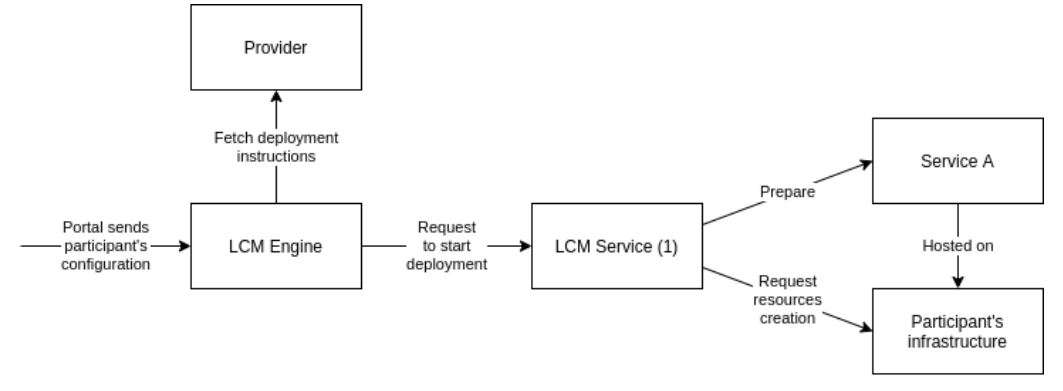
\includegraphics[width=\textwidth]{gfx/chapters/4_gaia-X/example_deployment.png}
  \caption{Beispiel einer Servicebereitstellung}
  \source{\cite{ORC2021}}
  \label{fig:gaia-x-example_deployment}
\end{figure}
Abbildung \ref{fig:gaia-x-example_deployment} verdeutlicht dieses Prinzip anhand eines Beispiels.
Ein Endnutzer übergibt seine gewünschte Konfiguration des Service A via Gaia-X Portal an die \ac{LCM} Engine.
Service A kann dabei allerdings nicht mit allen LCM Services bereitgestellt werden,
sodass der Nutzer sich für den \emph{\ac{LCM} Service (1)} entscheidet.
Die Engine fragt beim Provider nach der Bereitstellungsanweisung für den Service an,
welche nach Zusammenführung mit der Nutzerkonfiguration an den \ac{LCM} Service weitergeleitet wird.
Der \ac{LCM} Service sorgt für die tatsächliche Bereitstellung des Service A
und gibt den Endpunkt des Service an die Engine zurück \cite{ORC2021}.

\section{Sovereign Cloud Stack}
\label{sec:gaia-x-einbettung:scs}

\begin{figure}[h]
  \centering
  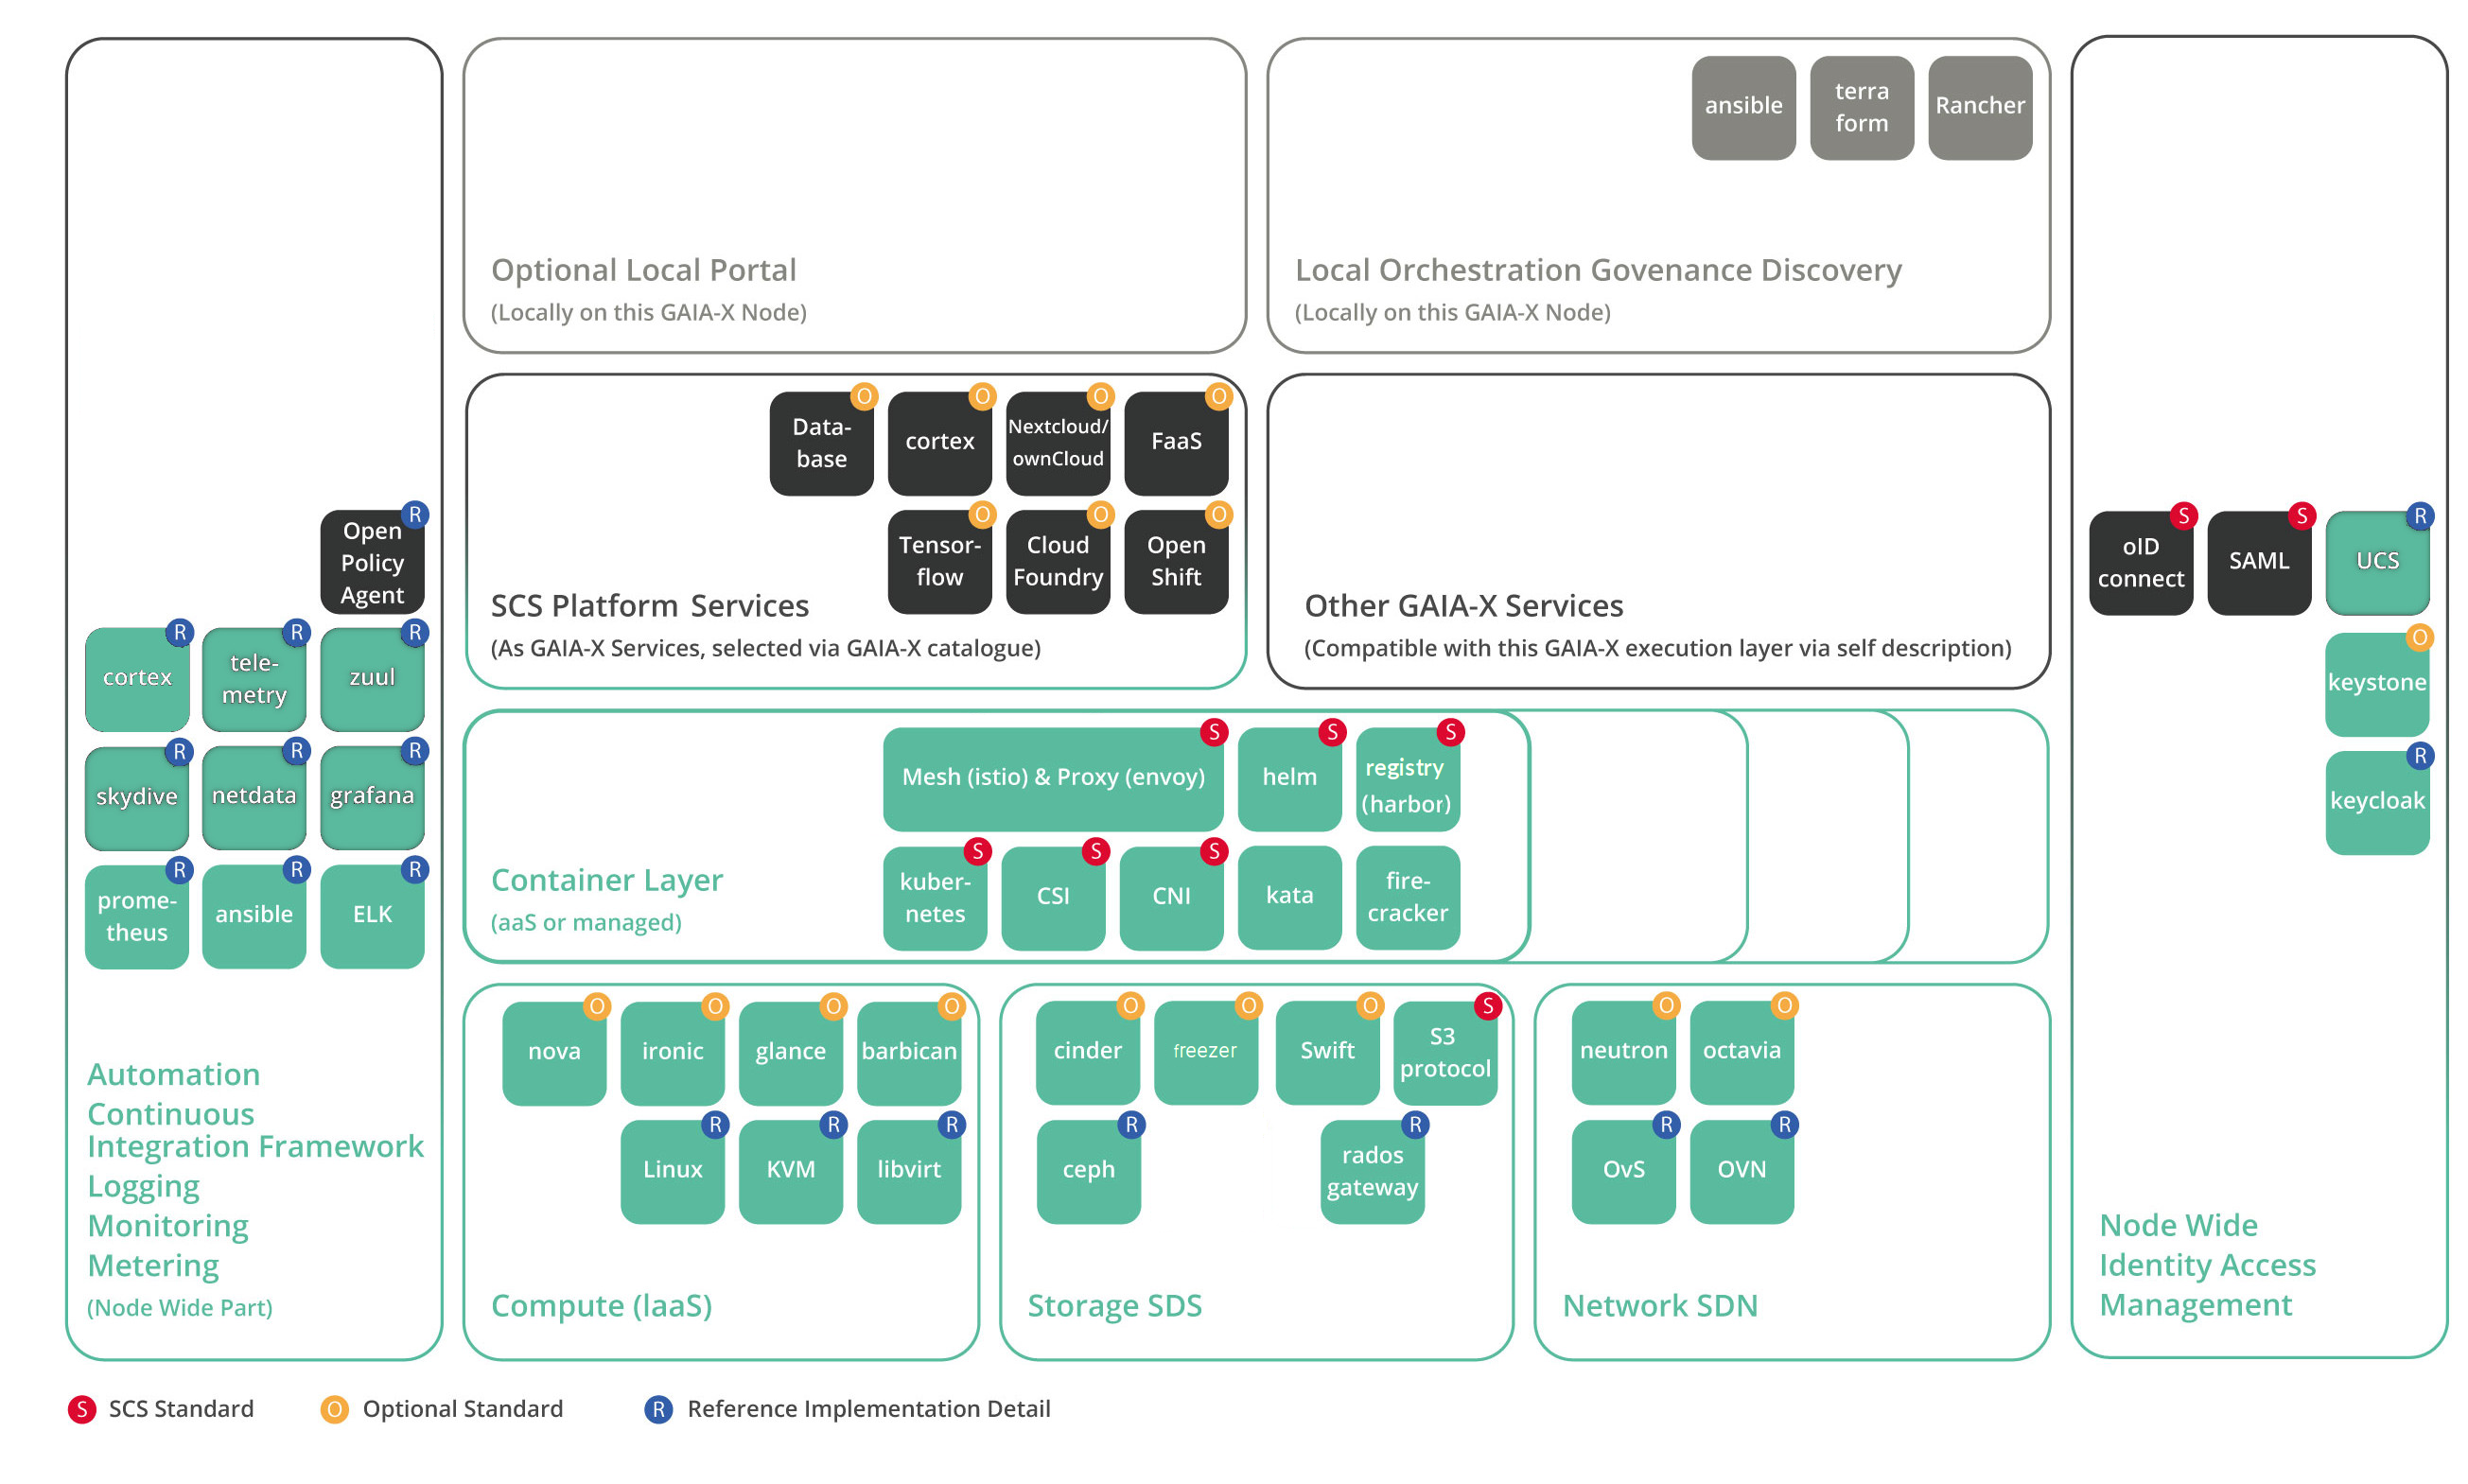
\includegraphics[height=0.71\textwidth]{gfx/chapters/4_gaia-X/scs_architecture.png}
  \caption{Architektur und Komponenten des Sovereign Cloud Stacks}
  \source{https://scs.community/assets/images/201001-SCS-4a.png}
  \label{fig:scs_architecture}
\end{figure}

\ac{SCS} ist ein Open-Source Projekt, um eine standartisierte und souveräne Plattform zu definieren, welche von 
existierenden und zukünfitgen Cloudprovidern genutzt werden soll. 
Ziel des Stacks ist ein Netzwerk von Anbietern, welche durch Nutzung von freier Software und gemeinsamer Standards,
eine interoperable, unabhängige Cloud schaffen \cite{Kagermann2021}.
Als technologischer Standpunkt dient \ref{fig:scs_architecture}, welches die geplante Architektur des \ac{SCS} zeigt. 
Grundlage des Stacks sind OpenStack Services, welche als OpenSource Projekt für Cloud-Computing Architektur entwickelt wurde.
Unterteilt wird dies in 3 grundlegende Bausteine: \textbf{Compute}, \textbf{Network} und \textbf{Storage},
welche als \ac{IaaS} Services definiert sind.
Die Openstack Services sollen als starke, multitenant fähige Basis für Kubernetes Cluster dienen. 
Der Hauptdienst soll Kubernetes as a Service darstellen, auf dem Provider intern ihre \ac{SaaS} aufbauen können \cite{scs}.
Darauf aufbauend wird ein Container Layer erstellt, welcher mit Hilfe von Containerruntimes
wie Docker oder 
Podman\footnote{Daemonlose Containerlaufzeitumgebung zur Verwaltung, Erstellung und Betrieb von Containern \cite{podman}.}
gesteuert werden soll \cite{scs}.

Services wie der in dieser Thesis entwickelte Chat \ac{SaaS} finden sich auf der übergeordneten Ebene \textbf{SCS Platform Services} wieder.
Für die Entwicklung des Rocket Chat \ac{SaaS} wurde diese Architektur als Grundbild genutzt, indem 
genannte Technologien des Stacks in der Implementierung berücksichtigt wurden.
\section{Erstellung der Testinfrastruktur}
\label{sec:gaia-x-einbettung:erstellung-testinfra}
Bei der Erstellung der Testinfrastruktur kam es zu einigen Einschränkungen im Vergleich zu bereits etablierten Hyperscaler Clouds,
da zum Zeitpunkt der Thesis nur Infrastruktur Services wie Netzwerke, DNS, \acp{VM} und Speicher
und kein Managed Kubernetes Service zur Verfügung stehen.
Durch die unterliegende Architektur des Gaia-X Providers kann allerdings bereits etablierte Software
zur Erstellung von Kubernetes Clustern genutzt werden.
Dazu wurde das Tool \textbf{Kubespray}\footnote{\url{https://github.com/kubernetes-sigs/kubespray}} genutzt,
welches mit Hilfe der Konfigurationssoftware \textbf{Ansible} und der \ac{IaC} Software \textbf{Terraform}
\acp{VM}, Netzwerk und Sicherheitsgruppen für die Kubernetes Knoten in der Cloud erstellt.

Aufgrund der zeitlichen Begrenzung der Testlizenz auf 30 Tage wurde jedoch zusätzlich eine lokal
testbare Version der benötigten OpenStack Services erstellt, 
Alle benötigen Services sowie eine vollwertiges Kubernetes Cluster werden in Containern bereitgestellt,
sodass diese lokal betrieben werden können.
Somit kann die Cloudunabhängigkeit von Kubernetes zum Vorteil für Entwickler und der schnellen Entwicklung genutzt werden.